\subsubsection{usergoal-ugCreateNewCrisisEvent}

\label{RE-use-case-ugCreateNewCrisisEvent}


The goal is to manage the creation of a new crisis event including all the necessary information.		  


\begin{usecase}
  \addheading{Use-Case Description}
  \addsingletwocolumnrow{Name}{ugCreateNewCrisisEvent}
  \addsingletwocolumnrow{Scope}{system}
  \addsingletwocolumnrow{Level}{usergoal}
  

\addrowheading{Primary actor(s)}
\addnumberedsinglerow{}{\msrcode{actCentralCoordinator[active]}}


\addrowheading{Secondary actor(s)}
\addnumberedsinglerow{}{\msrcode{actCommunicationCompany[active]}}
\addnumberedsinglerow{}{\msrcode{actFiremenCoordinator[passive]}}
\addnumberedsinglerow{}{\msrcode{actTowServiceCoordinator[passive]}}

\addrowheading{Goal(s) description}
\addsinglerow{The goal is to manage the creation of a new crisis event including all the necessary information.}

\addrowheading{Reuse}
\addnumberedsinglerow{}{\msrucname{oeAddNewCrisisEvent [1..*]}}
\addnumberedsinglerow{}{\msrucname{oeRequestCrisisEventLocation [1..*]}}
\addnumberedsinglerow{}{\msrucname{oeReceiveCrisisEventLocation [1..*]}}
\addnumberedsinglerow{}{\msrucname{oeCreateNewCrisisEvent [1..*]}}
\addnumberedsinglerow{}{\msrucname{oeMovePinOnMap [0..*]}}

\addrowheading{Protocol condition(s)}
\addnumberedsinglerow{}{
none.}

\addrowheading{Pre-condition(s)}
\addnumberedsinglerow{}{
none.}

\addrowheading{Main post-condition(s)}
\addnumberedsinglerow{}{
a dispatch order including the crisis event's information such as the id, map with pin, witness's phone number, etc. is sent to nearest, free Firemen Team and Tow Service Team.}

\addrowheading{Main Steps}
\addalphanumberedsinglerow{}{the actor \msrcode{actCentralCoordinator} executes the \msrucname{oeAddNewCrisisEvent} use case}
\addalphanumberedsinglerow{}{the actor \msrcode{actCentralCoordinator} executes the \msrucname{oeRequestCrisisEventLocation} use case}
\addalphanumberedsinglerow{}{the actor \msrcode{actCommunicationCompany} executes the \msrucname{oeReceiveCrisisEventLocation} use case}
\addalphanumberedsinglerow{}{the actor \msrcode{actCentralCoordinator} executes the \msrucname{oeMovePinOnMap} use case}
\addalphanumberedsinglerow{}{the actor \msrcode{actCentralCoordinator} executes the \msrucname{oeCreateNewCrisisEvent} use case}
\addrowheading{Steps Ordering Constraints}
\addnumberedsinglerow{}{step (a) must be executed first}
\addnumberedsinglerow{}{if step (c) then previously step (b)}
\addnumberedsinglerow{}{if step (d) then previously step (c)}
\addnumberedsinglerow{}{step (e) executed as last}
\addnumberedsinglerow{}{step (a), (b), (c), (e) must be executed at least once}

\addrowheading{Additional Information}
\addsinglerow{
none
}

\end{usecase} 


Figure \ref{fig:lu.uni.lassy.excalibur.group09.spec-RE-UCD-uc-ugCreateNewCrisisEvent}
Shows the ugCreateNewCrisisEvent use-case and its actors.

\begin{figure}[htbp]
\begin{center}

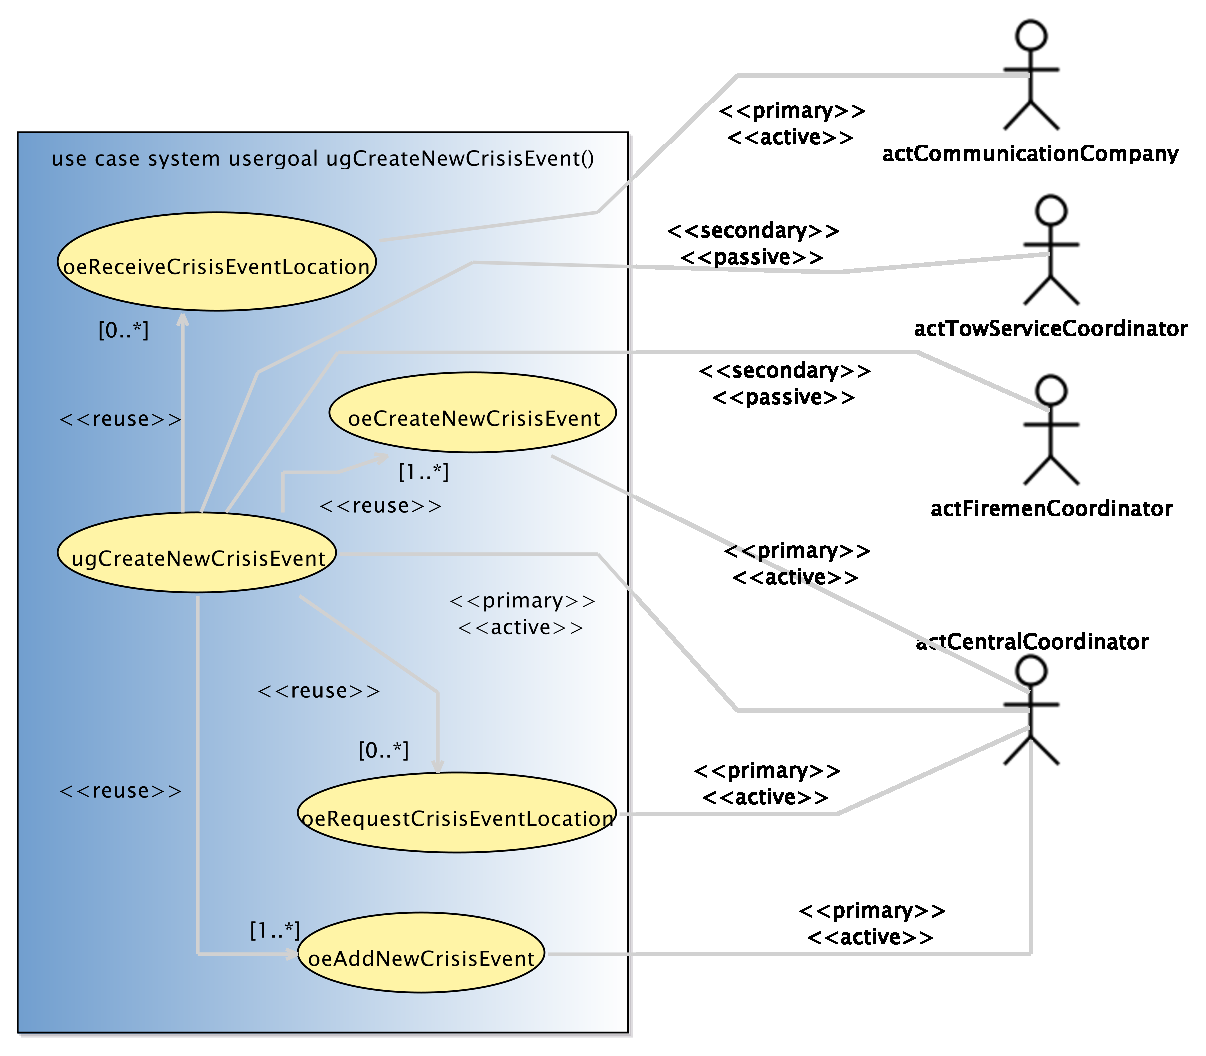
\includegraphics[
angle=0
,width=1.0\textwidth
]{./images-report-gen/usecase-model/usergoal/uc-ugCreateNewCrisisEvent.eps}
\end{center}
\caption[lu.uni.lassy.excalibur.group09.spec Use Case Diagram: uc-ugCreateNewCrisisEvent]{ugCreateNewCrisisEvent}
\label{fig:lu.uni.lassy.excalibur.group09.spec-RE-UCD-uc-ugCreateNewCrisisEvent}
\end{figure}
\vspace{0.5cm}
